\documentclass[11pt]{article}% uses letterpaper by default

%---------- Uncomment one of them ------------------------------
\usepackage[includeheadfoot, top=1in, bottom=1in, hmargin=1in]{geometry}

% \usepackage[a5paper, landscape, twocolumn, twoside,
%    left=2cm, hmarginratio=2:1, includemp, marginparwidth=43pt, 
%    bottom=1cm, foot=.7cm, includefoot, textheight=11cm, heightrounded,
%    columnsep=1cm, dvips,  verbose]{geometry}
%---------------------------------------------------------------
\usepackage{fancyhdr}
\renewcommand{\footrulewidth}{0.4pt}% default is 0pt
\usepackage{verbatim}
\usepackage{url}
\usepackage{cancel}
\pagestyle{fancy}
\usepackage{graphicx}
\usepackage{setspace}
\singlespacing
%\doublespacing
%\onehalfspacing
\usepackage{varwidth}
\usepackage{hyperref}
\usepackage{xcolor}

\newcommand{\degrees}{\ensuremath{^\circ}}
\newcommand{\arcmin}{\ensuremath{'}}
\newcommand{\arcsec}{\ensuremath{"}}
\newcommand{\hours}{\ensuremath{^\mathrm{h}}}
\newcommand{\minutes}{\ensuremath{^\mathrm{m}}}
\newcommand{\seconds}{\ensuremath{^\mathrm{s}}}

\newcommand{\s}[0]{\phantom{i}} %sets up \s command
\newcommand{\m}[0]{\phantom{abcde}} %sets up \m command
\providecommand{\e}[1]{\ensuremath{\times 10^{#1}}} %sets up \e command
\setlength{\parindent}{0.2in} %new paragraph indent
\usepackage{indentfirst} % indent the first paragraph of a section
\usepackage{amsmath,amssymb}
\usepackage{enumitem}

\lhead{Astronomy Lab II}
\rhead{Fall 2024}
\lfoot{Porter}
\rfoot{Wed 6-9pm}
\cfoot{\thepage}

%\newcommand{\exercisename}{7}
\begin{document}

\begin{center}
\huge{Lab 8: Thinking Like An Astronomer: Research, Data, and Peer Review}\\ \medskip \Large{November 6, 2024}
\end{center}

%\textcolor{red}{Lori: pick out a sample paper (hopefully a simple one; maybe a letter?) for everyone to look at. We should go over what their data is, the question(s) they're looking at and trying to answer (or science goals), use critical thinking to determine possible biases, discuss funding and potential implications for bias, how they conducted their investigation, whether it is a reliable source or not, etc. Lab questions should focus around these papers and questions: students should be able to identify good versus bad research sources, biases, aspects of scientific research, how things are published, how peer-review works, what a reputable journal is, pop science versus peer-reviewed research, what actual articles look like, etc.}

%From message to Chris: go over the scientific method and how science isn't a linear process, go over what publishing and peer-review is like, stem off into identifying reputable sources and when certain sources are appropriate. For example, I don't expect non-majors to browse and understand ADS, but rather find more reputable, easier-to-understand sources like astrobites? Do section on critical thinking, include things like identifying trends, correlation vs causation, identifying possible biases. 

%Goal is to teach that scientific research is actually incredibly complex and promote general skills interpreting data. 

%What does a good versus bad plot look like?

%Make some ridiculous plot example of two uncorrelated variables that look like they might have a relationship. Have them compare with a galaxy rotation curve plot like we did last week; why can we derive scientific conclusions from the rotation curves, but not the ridiculous plot?

%Look at some studies with funding bias, example of fossil fuel studies that are funded by Exxon? Election szn?

\section{Introduction: The Scientific Process (is non-linear!)}

What does astronomy research actually \textit{mean}? By now, you've probably learned that astronomy is about so much more than scientists looking at pretty pictures of space. However, we can't study planets, stars, and galaxies in a lab, and new scientific discoveries are \textit{complicated} processes that build off of years, if not decades, of previous work. So, what actually qualifies as scientific research, and how is it performed? What are astronomers doing day-to-day, and what counts as a 'discovery'? How can we connect this to daily life?

The purpose of this week's lab is to familiarize you with the process and challenges of conducting real research, how to interpret studies across all fields, how to convey information, and to use critical thinking. \textbf{These are all \textit{essential} skills to have, regardless of your major.} This lab will also ideally help you begin your final projects.

You've probably seen some form of the scientific process (or scientific method) in school before. This is a good place to start with how research is conducted. In general, the scientific process usually consists of several key steps:

\begin{enumerate}
    \item Ask a question/Identify a problem
    \item Construct a hypothesis or prediction
    \item Perform an experiment to test the hypothesis
    \item Analyze your data and results
    \item Create a conclusion
\end{enumerate}

 While this is a simplified view of the scientific process, you should see that it begins with asking questions. This is the process of \textbf{inquiry}. The \href{https://eric.ed.gov/?id=ED391690}{National Research Council} defines the process of inquiry to include asking questions, planning investigations, thinking critically and logically about relationships between evidence and explanations, and communicating scientific arguments. In essence, the process of inquiry describes the \textbf{thinking process} of a scientist and the path to the generation of new knowledge. Once one question has been answered, the process repeats, cyclically, as new questions arise. 

 \begin{figure}
     \centering
     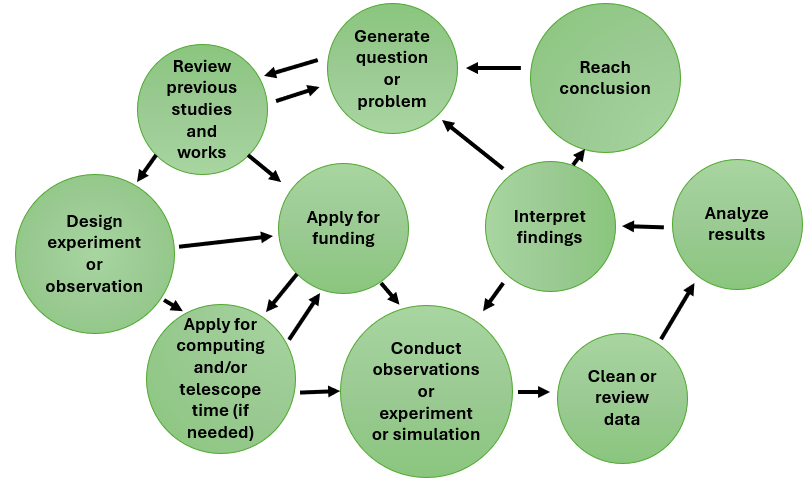
\includegraphics[width=0.75\linewidth]{Images/scientificmethod.png}
     \caption{A more realistic representation of the scientific method, particularly for astronomy. There are even more combinations and steps not listed here.}
     \label{fig:scientificmethod}
 \end{figure}

It’s important to note that the inquiry process is not linear and orderly, or even always successful -- scientists hit dead ends all the time in their research, or have to re-calculate and start over -- that's just part of doing science. Dr. Greg Bryan, the Chair of the Department of Astronomy, often refers to this as putting the "re" in "research."  Sometimes, the scientific process actually looks something like Figure~\ref{fig:scientificmethod}. %, either due to lack of sufficient data, insufficient quality of data, technological barriers, budget or time constraints, or other factors -- that’s just part of the process of doing science! 

\newpage

\textbf{Record the following in your lab write-up.}

\begin{enumerate}
\setcounter{enumi}{0}

\item What are some specific problems you anticipate could happen when doing astronomy research? List a few examples, and why these would make the process more complicated.
 
\end{enumerate}

\subsection{How Astronomers Actually Begin}

It's easy to say that the scientific process starts with a question or problem, but this can be a difficult step, especially for less experienced researchers. Let's determine what constitutes a good research question. \textbf{Record the following in your lab write-up:}

\begin{enumerate}
\setcounter{enumi}{1}

\item Using what you know about the scientific process from the last section, what are at least \textit{two} qualities a research question or problem needs to have in order to follow the scientific process?

%\textbf{The question must be something that can be tested or proved. The question or problem also needs to have some prior information so that we can determine \textit{how} to go about answering it.}
 
\end{enumerate}

In research, problems being investigated need to be something that can be tested: you must be able to perform some kind of experiment to generate data and lead to a conclusion. This is why questions such as "Do alternate Universes exist?" and "What happens inside a black hole?" are things that can't be reliably studied: there do not currently exist any methods to test these questions. Astronomers typically identify interesting topics to study, then apply for funding and resources (computing time, telescope time) to study the topic. These resources can be \textit{incredibly} competitive. 

\newpage

Let's do some quick math; \textbf{record the following in your lab write-up.}

\begin{enumerate}
\setcounter{enumi}{2}

\item According to \href{https://science.nasa.gov/mission/hubble/overview/hubble-by-the-numbers/}{NASA}, if you want to do science that requires observations from the Hubble Space Telescope, the odds of having your proposal selected are about 1 in 5, or 20\%. A \href{https://www.science.org/content/article/odds-improve-winning-nsf-grants-drop-applications-troubles-some-observers}{recent report} also showed that the success rate of getting funding from the National Science Foundation (NSF) is about 28\%. If an average astronomer needed to get both telescope time and funding, what are their odds of being successful at both? Assume both events are independent, and our average astronomer has one application to each. Is success likely to happen? \\ \textit{Hint}: from probability, multiply the probability of the first event times the probability of the second event.

%\textbf{Multiply 0.2 times 0.28. Should get 0.056, or 5.6\%. Not likely to happen.}
 
\end{enumerate}

Furthermore, there is rarely only one correct way to test a research question. Astronomy can be conducted through observations, direct measurements with a telescope, or through simulations and theory, where a developed computer program and/or framework of physics and mathematics can be applied to investigate a problem. Even within each of these methods, there are \textit{hundreds} of ways to approach specific problems. This is what makes research so broad, and why creativity is a key part of science! If it can be proven effective, a new method can provide a lot of new information. 

However, methods and research questions need to be based off of previous knowledge. Conducting good research that contributes to the world's knowledge uses work done by previous astronomers to build upon a knowledge basis: what methods do and don't work? What different ways can data and predictions be tested? Does one method provide different results from another, and why? True research starts with a comprehensive summary of the work that came before it and led to the question or problem being solved. 

\begin{enumerate}
\setcounter{enumi}{3}

\item \textbf{Follow the below steps in your lab write-up} to generate your own research question:
\begin{enumerate}
    \item What is something you've learned about in lecture or previous labs, but still have questions about? Briefly name the topic and explain what you \textit{do} know.
    \item What is your remaining question about the topic? How did your previous knowledge allow you to ask this?
    \item How do you think you could go about answering this question? You don't have to design your own experiment in detail, but provide a brief answer, whether you suggest using telescopes or looking to see what other researchers have found. Feel free to ask your instructor if you aren't sure how.
\end{enumerate}

\end{enumerate}

%%%%%%%%%%%%%%%% Section 2: Presenting and Understanding Data %%%%%%%%%%%%%%%%
\newpage

\section{Presenting and Understanding Data: A Picture is Worth a Thousand Words}

In this course, especially in recent labs, we've placed a LOT of focus, especially since Lab 4, on creating plots and graphs using data. While some of the software can be a challenge to learn, there's a reason astronomers generally prefer to show graphs and images where possible. After all, they do say a picture is worth a thousand words. 

As you might have noticed, learning to \textit{create} and \textit{read} graphs is an art of its own. There's more than one way to show data, and each method can tell you something different about the data. \textbf{Graphs are how we communicate data and scientific results}, so it's especially important to be able to read and interpret them correctly. This involves more than just being able to correctly label plot axes or read values off of a chart. Let's start thinking about this; \textbf{answer the following questions in your lab write-up.}

\begin{enumerate}
\setcounter{enumi}{4}
    \item What information should be conveyed in a plot? Why has your lab instructor required you to always include axis labels, units, and to use specific plot types? Be specific.

    %\textbf{A reader should be able to see the plot and draw a clear conclusion from it.}

    %\textbf{Necessary to interpret data!! }

    \item What can happen if something isn't included or labeled correctly?

    %\textbf{Data can be misinterpreted, harder to spot errors, etc}
\end{enumerate}

However, just because a plot \textit{looks} complete, that doesn't mean it is reliable. You've just learned that graphs are a form of communication in science, but just like face-to-face communication, the way data is represented can be misleading (sometimes intentionally). 

\begin{enumerate}
\setcounter{enumi}{6}

\item Look at Figure~\ref{fig:example_scatter_trend}.
    \begin{enumerate}
        \item Do you see a trend in the data? Draw an approximate trendline through the data.
        \item If your lab partner told you that this graph means that in recent years, the consumption of sugar has increased in many countries, would you agree with them? Why or why not?
        \item In your own words, describe what this data is showing. 
    \end{enumerate}
\end{enumerate}

\begin{figure}
    \centering
    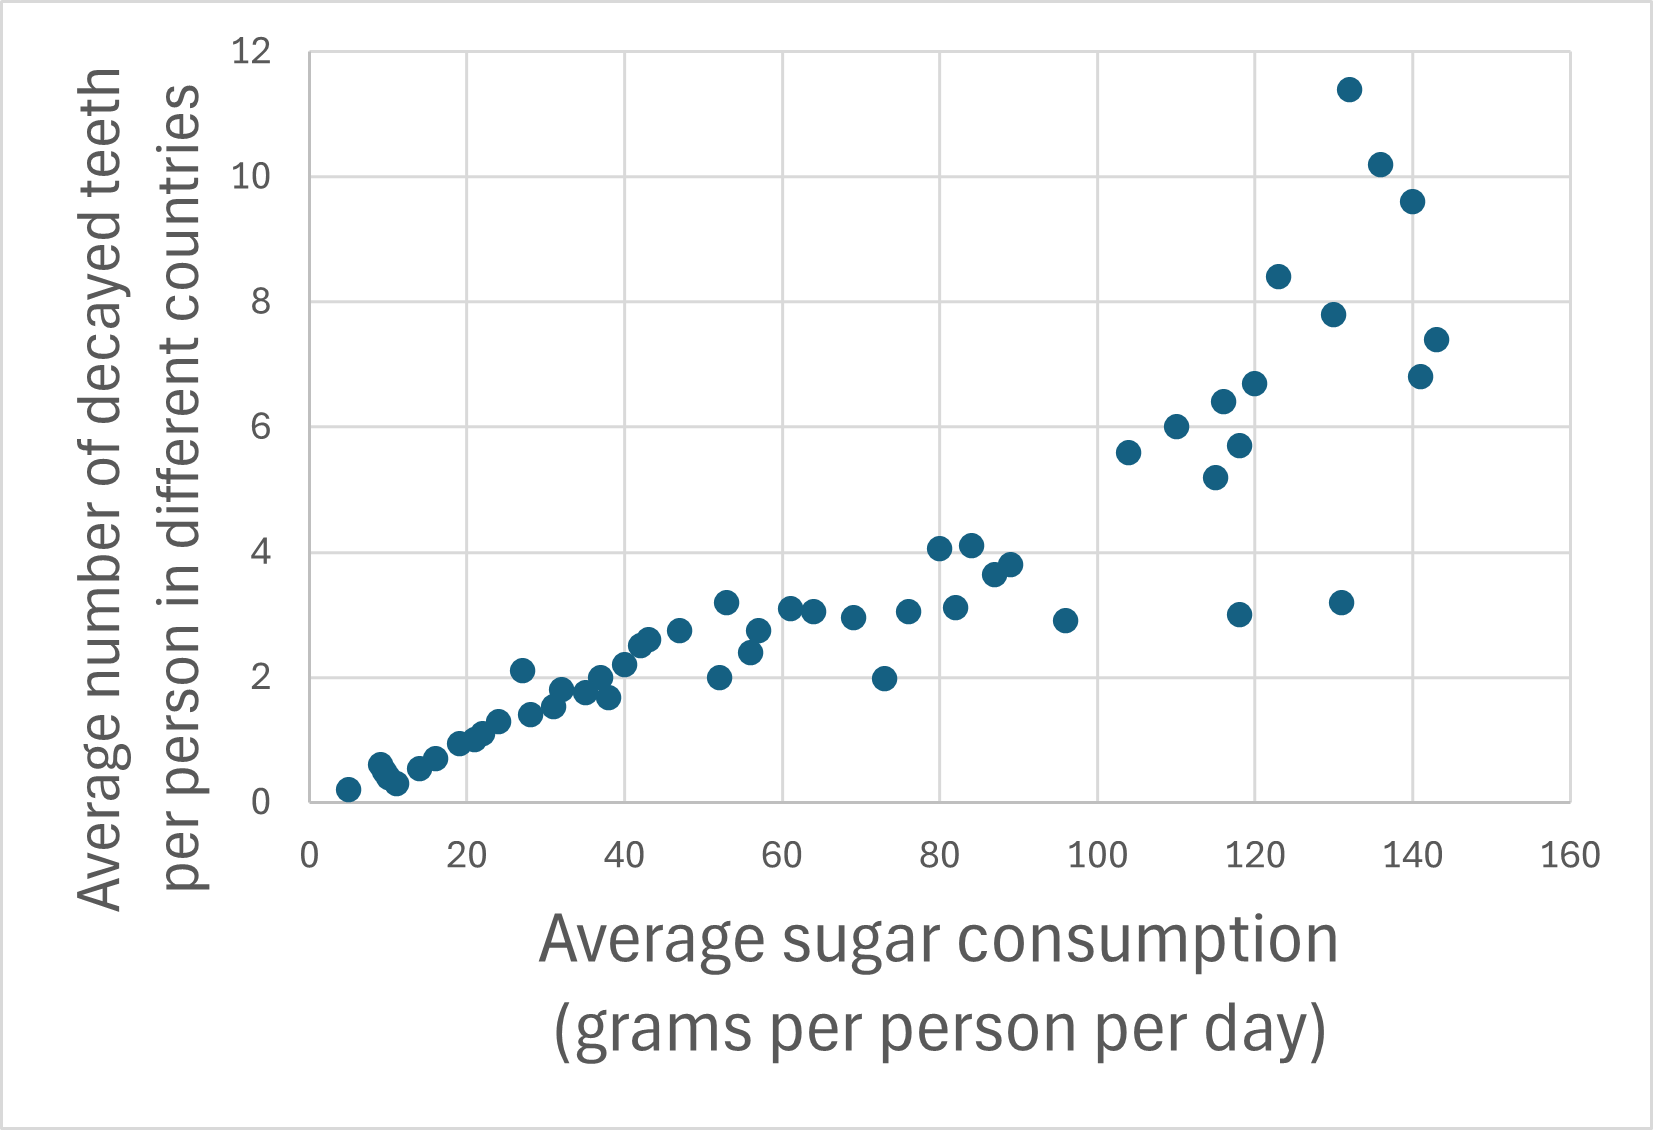
\includegraphics[width=0.5\linewidth]{Images/example_scatter_trend.png}
    \caption{ Figure for Question 7.}
    \label{fig:example_scatter_trend}
\end{figure}

\begin{figure}
    \centering
    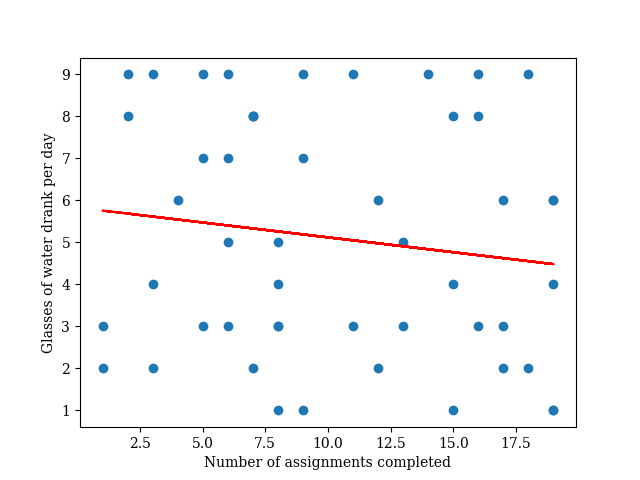
\includegraphics[width=0.75\linewidth]{Images/scatter_bad_trend.png}
    \caption{Figure for Question 8.}
    \label{fig:scatter_bad_trend}
\end{figure}

This is an example of a \textit{clear trend} being visible in data, and the last problem tested your ability to interpret what this trend means. Let's look at another example in Figure~\ref{fig:scatter_bad_trend}. 

\begin{enumerate}
    \setcounter{enumi}{7}
    \item What is the trendline of the data implying? What can you conclude from the way this data is presented to you?
    \item Ignore the trendline and focus on the data points themselves. Would you still agree with your original conclusion? Why or why not?
\end{enumerate}

\newpage

It's important to understand that just because a trendline \textit{can} be plotted onto data, it doesn't mean you should. This is applicable to other fitting functions, too, such as logarithms, polynomials, and exponentials. You can usually always fit these functions to data, but \textbf{you must always remember what information you want your graph to convey to a reader.} Even though the points of Figure~\ref{fig:scatter_bad_trend} are actually random, the trendline gives the impression that some relationship exists between the x and y variables, even though there isn't one: the number of assignments completed by a student is NOT correlated with the glasses of water drank per day. \href{https://www.xkcd.com/1725/}{This comic} is meant to be humorous, but has a lot of truth to it!

Finally, let's investigate how important it is to use the right visuals in a graph. While science has a reputation for only being about experiments and numbers, graphic design is an essential skill, too! \textbf{Every design choice should be justified and intentional.}

\begin{enumerate}
    \setcounter{enumi}{9}
    \item A few astronomy plots have been picked out for you. \textbf{In your write-up,} identify at least one design element that may not be the best choice to convey their results. You might have to look closely or discuss with other groups; there is at least one key element you should be identifying for each. (Note that 2 of 3 of these plots are published; suboptimal design doesn't necessarily mean bad science.)
    \begin{enumerate}
        \item \href{https://www.pnas.org/doi/10.1073/pnas.1812905116}{Plot A, scroll down to Figure 1}
        \item \href{https://earthobservatory.nasa.gov/blogs/elegantfigures/wp-content/uploads/sites/4/2010/08/npp_trend_original.png}{Plot B}
        \item \href{https://ibb.co/8DNLBgX}{Plot C}
    \end{enumerate}
\end{enumerate}
    
    %\item Example of a plot with no real or mispresentative trend.
    
    %\item Example of a plot with bad bounds/axes?
 
%\end{enumerate}

%%%%%%%%%%%%%%%% Section 3: Critical Thinking and Bias %%%%%%%%%%%%%%%%
\bigskip

\section{Importance of Critical Thinking}

Just as scientific processes follow some of the steps outlined in Figure~\ref{fig:scientificmethod}, in the previous section you used a process called \textbf{critical thinking} to determine whether certain design choices were effective at communication or not. Some of these answers may not have been immediately obvious to you, and required you to think a bit deeper, ask for help, or use new perspectives. This is why critical thinking is so essential: it is defined as \textbf{the analysis of facts to form a judgment.}

Critical thinking can require a bit more effort, especially in astronomy, but is part of being both a good scientist and communicator. Some examples of critical thinking are asking yourself questions such as:
\begin{itemize}
    \item Why does the author/person think this?
    \item What does this make me wonder?
    \item Why did this author/person choose to do this?
    \item Who is stating this?
    \item How could this be seen from another perspective?
    \item Can this be replicated/Would another method reproduce the same result?
    \item How could this be tested to see if it is true?
\end{itemize}

As we'll find out, critical thinking can be a key tool to interpreting research.

\subsection{Example: Correlation vs. Causation}

Often in class, we'll plot two different quantities to determine if a relationship between the variables exists. However, we need to be extra cautious about interpretations here, and is where critical thinking can come in handy. You can find \textbf{correlation} between two variables, meaning there appears to be some trend, but this does not always mean \textbf{causation}, that there is an inherent link between the two variables. \textbf{Complete the following in your lab write-up.}

\begin{enumerate}
\setcounter{enumi}{10}
    \item Look at Figure~\ref{fig:correlation_causation}, which contains two separate plots.
    \begin{enumerate}
        \item Does panel A show correlation, causation, or both? How do you know?
        \item Assume each galaxy in panel B has a \textit{constant luminosity,} or \textit{constant absolute magnitude}. Does panel B show correlation, causation, or both? How do you know?
    \end{enumerate}

    \item Think back to last lab, where we plotted galaxy rotation curves (radius on the x-axis and orbital velocity on the y-axis) to infer the presence of dark matter. Why were able to make \textit{reliable} scientific conclusions from that plot, but not a plot such as Figure~\ref{fig:scatter_bad_trend}?

\end{enumerate}

\begin{figure}
    \centering
    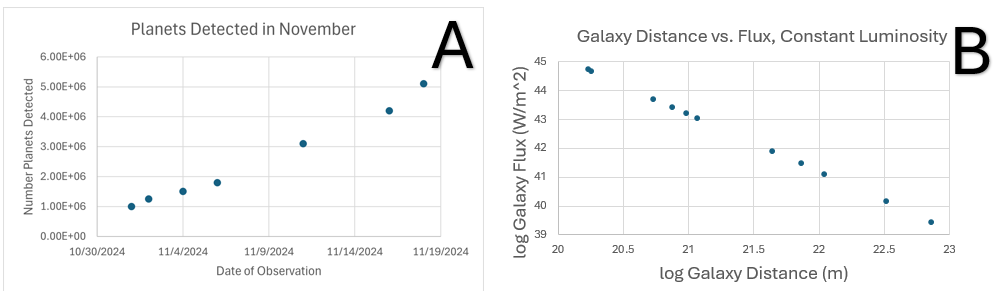
\includegraphics[width=\linewidth]{Images/correlation_causation.png}
    \caption{Figure for Question 12.}
    \label{fig:correlation_causation}
\end{figure}


%%%%%%%%%%%%%%%% Section 4: Publishing and Peer-Review %%%%%%%%%%%%%%%%
\bigskip 

\section{Publishing and Peer-Review}

The previous sections of this lab have focused on the processes driving research, creating and reading results, and how to critically think about such results. These are all key components that must be understood in science, and largely make up how most science (including astronomy) is done. \textbf{So, how do professional astronomers follow all of these guidelines when making their results available to the world?} When \textit{can} results be published? \textit{Where} are they published?

\medskip

The first thing to note is that \textit{not all research is publishable.} Publishing research is typically how astronomers get credit for their work, which means the research is submitted to a journal, a professional collection of related research intended for use by students and other researchers. Typically, journals will only publish research they consider to be \textbf{novel}, which means that the research is new or original, providing some new contribution to the field. Repeating a previous experiment in the exact same methods and getting the exact same results is not usually considered novel.

\medskip

Once the research is complete and results are written up, the authors make a submission to the journal. To uphold research standards and determine the validity of the research and arguments being made, reliable journals use a process called \textbf{peer-review}. In this process, the editor of the journal will send the article to an astronomer considered an expert in the topic of the paper, where this astronomer is now known as the reviewer. The reviewer, anonymous to the authors, conducts a thorough analysis of the paper and produces a report with comments on the research, which is sent to the editor, along with a recommendation for publishing (or not). This recommendation usually has one of four outcomes: accepted (no revisions necessary), minor revisions (some small points to correct), major revisions (significant changes requested), or rejection. This is forwarded to the authors for further changes. If a paper is rejected, it generally can't be re-submitted to the same journal. 

\medskip

Peer-review isn't perfect, as many requested changes, publishing recommendations, and preferences can be incredibly subjective, but it significantly increases a source's credibility, as it has been reviewed by other experts in the field. We'll do a peer-review activity of final project progress in our next lab; you may find some of your peers' comments to be helpful! Because research papers can be incredibly dense and difficult to understand, I highly recommend checking out \href{https://astrobites.org/category/daily-paper-summaries/}{Astrobites} for your research projects; Astrobites contains reviews of research that aim to be more easily understood, written by graduate students for undergraduates.


\begin{enumerate}
\setcounter{enumi}{12}

\item Visit the website for the \href{https://academic.oup.com/mnras}{Monthly Notices of the Royal Astronomical Society} or \href{https://iopscience.iop.org/journal/0004-637X}{The Astrophysical Journal}. If you scroll down, you should find recently published research articles. Pick two; you do NOT need to understand anything!

\begin{enumerate}
    \item Include the titles of the papers you chose.
    \item Scroll through both; what do both papers have in common with how they are organized (in terms of sections)? If you wanted to \textit{quickly} find the key points of the paper, what one or two sections would be most helpful?
\end{enumerate}

\item Briefly look at \href{https://www.timesnownews.com/technology-science/explainers/what-are-white-holes-and-do-they-really-exist-explained-article-106564032}{this article.} Do you think this is considered a reliable source? Why or why not?
 
\item Why is a peer-reviewed \textit{generally} more trustworthy?

\end{enumerate}


%%%%%%%%%%%%%%%% Section 5: Wrapping up %%%%%%%%%%%%%%%%
\bigskip

\section{Wrapping Things Up}
\begin{enumerate}
\setcounter{enumi}{15}

\item When we say that published research is "novel", what does this mean? Explain in \textit{your own words.}

\item How can critical thinking be applied in your daily life, and how might an astronomer use it? Support your answer with examples.

\item In what situations might you need to read and understand a graph? Can you think of any real-life consequences if you misinterpret the graph in this scenario?

\item In your opinion, what seems to be the hardest part about conducting scientific research, and why? Is there a specific part of the process that gives you the most hesitation or confuses you?
 
\end{enumerate}

\bigskip


\begin{center}
    {\Large{\textbf{*****If you have not done so already:*****}}} \\
    
     \bigskip
    
     \Large{Develop a final project idea and determine whether you will do a creative project or not. Submit it for approval in the \href{https://docs.google.com/spreadsheets/d/1pQL9EKsNcH44vz1XoKthK_Kj-6gCoj2f-hyi6Vgz924/edit?usp=sharing}{class spreadsheet}. You will probably need to request edit access, but I will approve it within a few hours, if not sooner.}

     \Large{If you need help, see the previous emails and files on Courseworks, come talk to me, or send me an email.}

     \bigskip

     \Large{\textbf{This \textit{MUST} be completed before our next lab. You will be unable to complete Lab 9 without this.}}
\end{center}



\end{document}

